\documentclass{article}

\usepackage{ctex}
\usepackage[top=0.7in,bottom=0.7in,left=0.5in,right=0.5in]{geometry}
\usepackage{array}
\usepackage{multirow}
\usepackage{graphicx}
\usepackage{subfigure}
\usepackage{fancyhdr}
\usepackage{lastpage}
\usepackage{extramarks}
\usepackage{amsmath}
\usepackage{listings}
\usepackage{fontspec}
\newfontfamily\consolas{Consolas}
\usepackage{xcolor} % 定制颜色
\definecolor{mygreen}{rgb}{0,0.6,0}
\definecolor{mygray}{rgb}{0.5,0.5,0.5}
\definecolor{mymauve}{rgb}{0.58,0,0.82}
\lstset{ %
backgroundcolor=\color{white},      % choose the background color
basicstyle=\footnotesize\ttfamily,  % size of fonts used for the code
columns=fullflexible,
tabsize=4,
breaklines=true,               % automatic line breaking only at whitespace
captionpos=b,                  % sets the caption-position to bottom
commentstyle=\color{mygreen},  % comment style
escapeinside={\%*}{*)},        % if you want to add LaTeX within your code
keywordstyle=\color{blue},     % keyword style
stringstyle=\color{mymauve}\ttfamily,  % string literal style
frame=single,
rulesepcolor=\color{red!20!green!20!blue!20},
% identifierstyle=\color{red},
language=c++,
}

\newcommand{\hmwkTitle}{哈夫曼编码压缩、解压文件\ 实验报告}
\newcommand{\hmwkClass}{数据结构}
\newcommand{\hmwkClassInstructor}{}
\newcommand{\hmwkAuthorName}{毛子恒\ 李臻\ 张梓靖}

\pagestyle{fancy}
\lhead{\hmwkAuthorName}
\chead{\hmwkClass\ : \hmwkTitle}
\rhead{\firstxmark}
\lfoot{\lastxmark}
\cfoot{\thepage}
\renewcommand\headrulewidth{0.4pt}
\renewcommand\footrulewidth{0.4pt}

\title{\hmwkClass\ :\hmwkTitle}
\author{\hmwkAuthorName}

\setcounter{tocdepth}{1}

\begin{document}

\maketitle

\section*{小组成员}

\setlength{\tabcolsep}{9mm}
{
    \begin{table}[htbp]
        \centering
        \begin{tabular}{llll}
            班级:2019211309 & 姓名:毛子恒 & 学号:2019211397 & 分工:代码\ 文档   \\

            班级:2019211310 & 姓名:李臻   & 学号:2019211458 & 分工:测试\ 文档   \\

            班级:2019211308 & 姓名:张梓靖 & 学号:2019211379 & 分工:可视化\ 文档 \\
        \end{tabular}
    \end{table}
}

\tableofcontents
\newpage

\section{需求分析}

\subsection{题目描述}

对于一个指定的文件,应用哈夫曼编码压缩文件,或者对本程序生成的压缩文件进行解压。

\subsection{输入描述}

程序从给定的二进制文件中读入数据。

\subsection{输出描述}

程序向给定的二进制文件中输出结果,向标准输出中输出提示。

压缩文件分为若干个部分,每个部分包含如下信息:

\begin{enumerate}
    \item 原字符串中包含的不同字符的个数;
    \item 哈夫曼树中每个节点存储的字符(非叶结点不存储字符)、结点左右孩子的序号;
    \item 原字符串的长度、压缩后位串的长度;
    \item 编码后的位串。
\end{enumerate}

输出分为五种情况:

\begin{enumerate}
    \item 输入合法,程序正常运行结束,此时结果存储在给定的二进制文件中,并在标准输出中打印提示信息。
    \item 输入不合法,程序向标准输出打印错误信息,并且要求重新输入或异常退出。
    \item 程序发生运行时错误,比如内存分配失败、指定的输入/输出文件无法打开。此时程序没有输出。
\end{enumerate}

关于更多细节请参考第5节。

\subsection{样例输入输出}

由于压缩后的二进制文件难以阅读,输入文件均以文本文件展示,压缩文件通过转换程序(testing/bit2string.c)转化成容易阅读的形式展现在本实验报告中,将不同数据以空格或换行符分隔,原本按每8位存储的位串转化成01字符串。

\subsubsection{样例输入输出1}

压缩。

【输入】(samples/sample1.in)

\begin{lstlisting}[
    basicstyle=\small\consolas]
aaababcd
\end{lstlisting}

【输出】(samples/sample1.out)

('\#'后的内容为注释)

\begin{lstlisting}[
    basicstyle=\small\consolas]
4     #出现的不同字符的个数/哈夫曼树叶结点的个数
c     #一个叶结点,其中存储字符c,没有左右孩子 
d
b
a
1 2   #一个非叶结点,不存储字符,左右孩子分别是1、2
3 5
4 6
8 2   #原串的长度,压缩后字符串的长度(2个字节)
0001001011011100 #压缩后的位串
\end{lstlisting}

\subsubsection{样例输入输出2}

压缩。

【输入】(samples/sample2.in)

\begin{lstlisting}[
    basicstyle=\small\consolas]
!#$""$#$"$$"!!"!$$#"$#"$"$!$#$!"!$!#"#!""#"!!!#"##"!$$$"#"$"$"$#!$$"$#!"#$##!!"#"#!!##!#$"!""$!"!#$$
\end{lstlisting}

【输出】(samples/sample2.out)

\begin{lstlisting}[
    basicstyle=\small\consolas]
4
#
!
"
$
1 2
3 4
5 6
100 25
010011101011001110111110010110011111001011001011101101110011011001110100100001101000100101010010000010011111111000
10111011101100011111101100011000110000010110001000010100000100111001101011011001001111
\end{lstlisting}

\subsubsection{样例输入输出3}

压缩。

【输入】(samples/sample3.in)

\begin{lstlisting}[
    basicstyle=\small\consolas]
1>8#2$'&'-).1%2/1:)/,8;2!3>(/69",#&7;>#$</%'=-=>+2#5&>!)5;(<96&;>0,7,;:/.)7$$/%5-(67933<(';==4464!12
\end{lstlisting}

【输出】(samples/sample3.out)

\begin{lstlisting}[
    basicstyle=\small\consolas]
29
"
+
0
.
:
8
-
5
9
<
!
4
3
%
)
'
&
$
#
=
7
6
1
,
(
2
>
;
/
1 2
3 30
4 5
6 31
7 8
9 10
11 12
13 14
15 32
16 17
18 19
20 21
22 23
24 25
26 33
27 34
28 35
29 36
37 38
39 40
41 42
43 44
45 46
47 48
49 50
51 52
53 54
55 56
100 60
111110100001101101100101101011000110011100001010101101011101111110101001010001111110111110110100000000011001100010
100101010001000001100011110011100011110000011011110011110101100100110111101001111100010101110001110001010111000100
001111100101101101011110010100100101011001011011000010111101110111101100101100100001110000011101000001101011111000
101110101101110111010110101000101010101101010000111110111010111010100101000111100011100001101110011100100111001111
110100111001011111001000
\end{lstlisting}

\subsubsection{样例输入输出4}

解压。(对应样例1)

【输入】

\begin{lstlisting}[
    basicstyle=\small\consolas]
4
c
d
b
a
1 2
3 5
4 6
8 2
0001001011011100
\end{lstlisting}

【输出】

\begin{lstlisting}[
    basicstyle=\small\consolas]
aaababcd
\end{lstlisting}

\subsubsection{样例输入输出5}

解压。(对应样例2)

【输入】

\begin{lstlisting}[
    basicstyle=\small\consolas]
4
#
!
"
$
1 2
3 4
5 6
100 25
010011101011001110111110010110011111001011001011101101110011011001110100100001101000100101010010000010011111111000
10111011101100011111101100011000110000010110001000010100000100111001101011011001001111
\end{lstlisting}

【输出】

\begin{lstlisting}[
    basicstyle=\small\consolas]
!#$""$#$"$$"!!"!$$#"$#"$"$!$#$!"!$!#"#!""#"!!!#"##"!$$$"#"$"$"$#!$$"$#!"#$##!!"#"#!!##!#$"!""$!"!#$$
\end{lstlisting}

\subsection{程序功能}

对于压缩过程,程序构造哈夫曼树并且对文件进行压缩,将需要的解码信息和压缩后的位串保存到压缩文件中。

对于解压过程,程序从压缩文件中读入解码信息和位串,并利用哈夫曼树进行解压。

\section{概要设计}

\subsection{问题解决的思路}

构造哈夫曼树进行压缩、解压过程。

\subsection{哈夫曼编码的设计}

\begin{lstlisting}[language={C},
    numbers=left,
    numberstyle=\tiny\consolas,
    basicstyle=\small\consolas]
// 数据对象
typedef struct node
{
    char data;
    int cnt;
    short parent, lc, rc; // 哈夫曼树双亲、孩子结点的下标
} Node;

/*
 * 操作:编码
 * 前件:inputFile和outputFile分别指向输入、输出文件
 * 后件:将编码结果输出到outputFile指向的文件中
 */
void encode(FILE * inputFile, FILE * outputFile);

/*
 * 操作:解码
 * 前件:inputFile和outputFile分别指向输入、输出文件
 * 后件:将解码结果输出到outputFile指向的文件中
 */
void decode(FILE * inputFile, FILE * outputFile);
\end{lstlisting}

\subsection{主程序的流程}

\begin{enumerate}
    \item 获取输入,判断是否合法
    \item 如果合法,则调用压缩/解压函数
\end{enumerate}

\subsection{各程序模块之间的层次关系}

程序模块层次关系图如图1。

\begin{figure}[htbp]

    \centering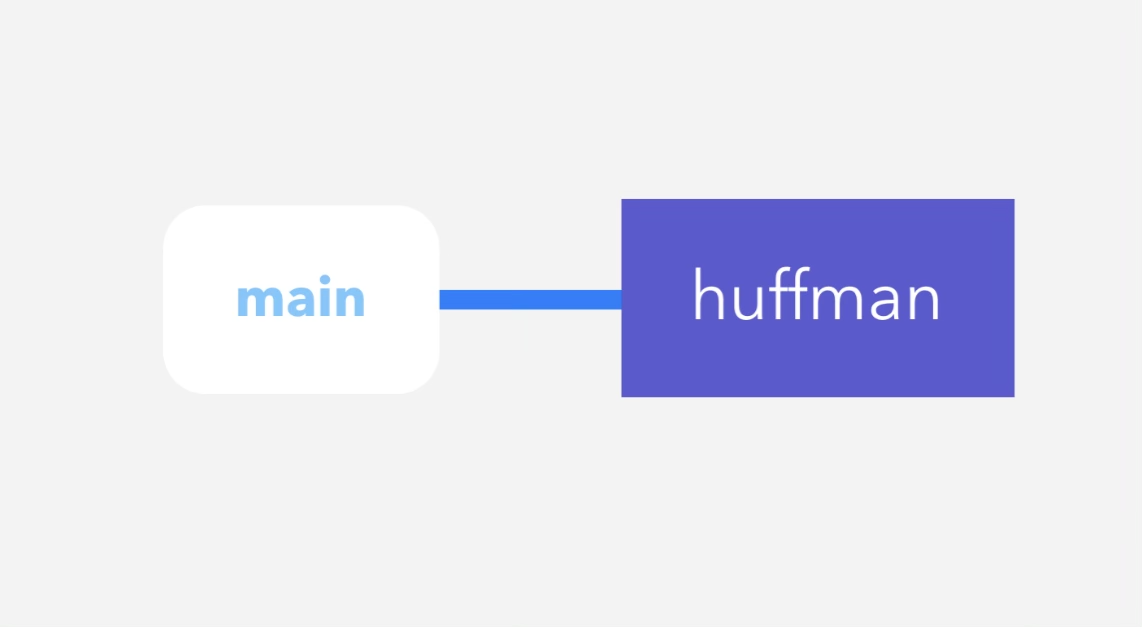
\includegraphics[width=0.4\textwidth]{./Images/pic4_2_1.png}

    \caption{程序模块层次关系}

\end{figure}

\section{详细设计}

\subsection{哈夫曼编码的实现}

哈夫曼编码的设计中基本操作的伪代码算法如下:

\begin{lstlisting}[language={C},
    numbers=left,
    numberstyle=\tiny\consolas,
    basicstyle=\small\consolas]
void encode(FILE * inputFile, FILE * outputFile)
{
    while (true)
    {
        从inputFile读入长度最长为1024字符串
        如果读到文件结束,退出循环
        cnt数组用来记录各个字符出现的次数,将其初始化
        统计各个字符出现次数(权值)
        按照权值从大到小对cnt数组排序
        从前往后,找到字符串的字符集的大小,设为tot
        创建tot个哈夫曼树叶结点(哈夫曼树采用顺序存储,权值小的字符在前)
        创建tot-1个非叶节点:
        t1 <- 1 目前没有双亲节点的权值最小的叶节点的下标
        t2 <- tot + 1 目前没有双亲节点的权值最小的非叶节点的下标
        for (int i = tot + 1 to 2 * tot + 1)
        {
            在t1、t1+1、t2、t2+2四个结点中选取权值最小的两个结点
            创建新的结点,左孩子和右孩子为刚刚选取的节点
            更新两个结点的双亲以及相应的指针
        }
        将tot写入文件
        将哈夫曼树叶节点存储的字符依次写入outputFile
        将哈夫曼树非叶节点的左右孩子结点的下标依次写入outputFile
        将原字符串的长度写入outputFile
        for (int i = 1 to tot)
        {
            从叶结点开始,逆向求每个字符的哈夫曼编码,作为'0'/'1'字符串写入tempString
            在huffmanCode数组(编码表)中分配位置,拷贝编码
        }
        将原字符串按照编码表编码,将编码结果写入tempString字符串中
        将tempString字符串的长度补全到8的倍数
        将tempString字符串每8个字符压缩到一个字节,写入到outputString中
        将编码后的字符串长度写入outputFile
        将outputString写入outputFile
        释放huffmanCode的空间
    }
}
void decode(FILE * inputFile, FILE * outputFile)
{
    while (true)
    {
        从inputFile读入tot
        如果读到文件结束,退出循环
        读入tot个叶节点的信息,复原哈夫曼树
        读入tot-1个非叶节点的信息,复原哈夫曼树
        读入原字符串的长度和编码后字符串的长度
        读入编码后的字符串inputString
        cur <- 2 * tot - 1 指针,表示当前在哈夫曼树中的结点下标
        for (int i = 0 to n-1)
        {
            for (int j = 0 to 7)
            {
                获取当前位的值temp
                if (temp)
                    cur指向当前结点的右孩子
                else
                    cur指向当前结点的左孩子
                if (找到了叶节点)
                {
                    将解码出的字符写入到outputFile
                    if (解码完了所有字符)
                        break;
                    cur恢复指向根结点
                }
            }
        }
    }
}
\end{lstlisting}

\subsection{函数的调用关系图}

函数调用关系图如图2。

\begin{figure}[htbp]

    \centering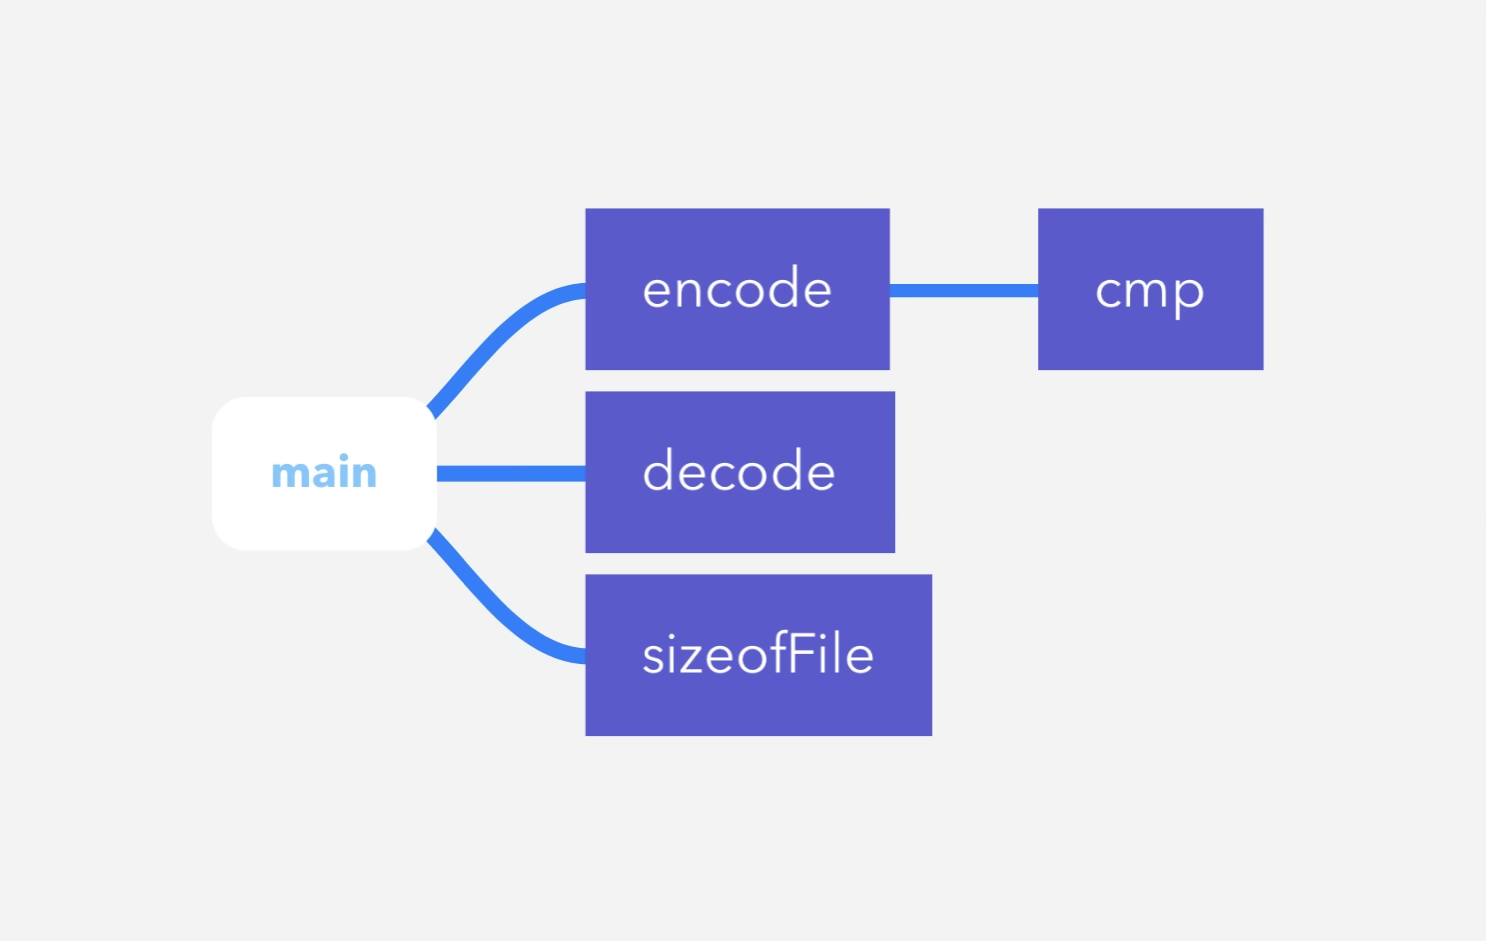
\includegraphics[width=0.4\textwidth]{./Images/pic4_2_2.png}

    \caption{函数调用关系图}

\end{figure}

\section{调试分析报告}

\subsection{调试过程中遇到的问题和思考}

由于对二进制文件的输入、输出不熟悉,曾尝试使用printf和scanf函数进行输入输出,了解相关知识后改为调用fread和
fwrite函数。

在解码的过程中feof函数经常出现探测文件末尾不准确,故改为判断fread函数是否为0来结束循环。

在构造哈夫曼树的过程中由于判断条件过于复杂,出现错误;改为了更简洁的判断条件。

在写入到压缩文件之前,压缩码需要以'0'/'1'字符串的形式存储,否则调用各种字符串函数会出现错误。

编码以8位压缩到一个字节当中,写入和读取的时候注意高低位的顺序。

\subsection{设计实现的回顾讨论}

编码是每次从二进制文件中读入1024个字节,创建编码表并且压缩。

由于哈夫曼树结点数较少,所以存储下标时采用short类型,写入压缩文件时可以节省空间。

对于没有出现过的字符显然不需要编码。调用库函数qsort对权值进行排序。

哈夫曼树采取顺序存储结构,前$n$个结点为叶节点,之后$n-1$个结点为非叶节点,每次构造新的非叶节点时只需要比较
叶节点中权值最小的两个结点和非叶节点中权值最小的两个结点,从中挑出权值最小的两个结点即可,使得查找结点的时间
复杂度降低到$O(1)$

压缩后的串为一个01串,将其每8位压缩到一个字节并写入压缩文件。

对于只有一种字符的情况,由于无法建立哈夫曼树,所以压缩文件中只存储tot、该字符、原字符串的长度。编码和解码是均
对这种情况特殊处理。

\subsection{算法复杂度分析}

encode,decode函数的复杂度为$O(len)$,其中$len$为字符串长度。

主函数的时间复杂度为$O(1)$,整体时间复杂度为$O(len)$。

\subsection{改进设想的经验和体会}

\subsubsection{改进1}

可以通过进一步压缩位(比如去掉一定为0的某些字节)来使得压缩率更高,但是编程复杂度会显著提高。

\subsubsection{改进2}

可以判断如果压缩率大于1,则直接写入原文件。

\section{用户使用说明}

使用gcc编译生成可执行文件。

\begin{lstlisting}[language={bash},
    basicstyle=\small\consolas]
gcc -o main -std=c11 main.c huffman.c
\end{lstlisting}

执行可执行文件:

\begin{lstlisting}[language={bash},
    basicstyle=\small\consolas]
./main
\end{lstlisting}

在Windows cmd下:

\begin{lstlisting}[language={bash},
    basicstyle=\small\consolas]
main
\end{lstlisting}

之后将数据写入到指定文件中,可以通过标准输入选择选项,也可以通过执行可执行文件时传递参数来选择选项:

\begin{enumerate}
    \item 如果执行可执行文件时没有传递参数,则可以根据标准输入的提示选择压缩/解压功能,以及指定输入和输出文件的位置
    \item 执行可执行文件时传递的参数:第一个参数为1或2,表示选择压缩/解压,之后两个参数分别为输入文件的路径和输出文件的路径,例如,执行
\begin{lstlisting}[language={bash},
    basicstyle=\small\consolas]
./main 1 ./input.in ./output.out
\end{lstlisting}
    表示执行压缩功能,输入文件为本目录下的input.in,输出文件为本目录下的output.out
\end{enumerate}

通过标准输出打印提示信息。如果输入合法并且程序正常运行结束,主函数返回值为0。

\section{测试结果}

测试环节分为三个步骤。

\subsection{测试第一部分}

对1.4节给出的样例进行测试。

\subsection{测试第二部分}

测试边界条件。

【输入】(samples/sample4.in)

(空文件)

【输出】(samples/sample4.out)

(空文件)

【输入】(samples/sample5.in)

文件内容为1000000个字符a

【输出】(samples/sample5.out)

压缩结果为一个8873字节的二进制文件。

【输入】

上一个例子的输出。

【输出】(samples/sample6.out)

解压与sample5.in相同。

\subsection{测试第三部分}

测试在macOS\ Big\ Sur\ 11.0.1下进行。

在$len<=10$,$len<=100$,$n<=1000000$的范围下分别随机生成1000组测试数据,进行压缩和解压操作,并且比对解压结果和原始输入是否相同。

3000组数据中没有出现错误。

数据生成程序(testing/data.cpp)如下:

\begin{lstlisting}[language={C++},
    numbers=left,
    numberstyle=\tiny\consolas,
    basicstyle=\small\consolas]
#include <bits/stdc++.h>
using namespace std;

int main(int argc, char *argv[])
{
    srand(time(0));
    FILE *file = fopen("./raw.in", "wb");
    int n = atoi(argv[1]), m = atoi(argv[2]);
    for (int i = 1; i <= n; ++i)
        fprintf(file, "%c", rand() % m + 32);
    fclose(file);
    return 0;
}
\end{lstlisting}

传入两个参数,第一个参数是字符串的长度,第二个参数是字符集的大小。

比对脚本(testing/chk.sh)如下:

\begin{lstlisting}[language={bash},
    numbers=left,
    numberstyle=\tiny\consolas,
    basicstyle=\small\consolas]
for i in {1..100}
do
    sleep 1
    ./data 100000 5
    ./main 1 raw.in encode.out
    ./main 2 encode.out decode.out
    if ! diff raw.in decode.out
    then
        break
    fi
    echo "Correct"
done
\end{lstlisting}

\section{可视化}

随机生成若干组数据,使用该程序进行压缩,记录不同数据规模下的平均压缩率,并且使用JavaScript将结果可视化。

比对脚本(testing/test.py)如下:

\begin{lstlisting}[language={python},
    numbers=left,
    numberstyle=\tiny\consolas,
    basicstyle=\small\consolas]
import os
import time

with open("./result.txt", "w") as file:
    for i in (10, 30, 50, 100, 500, 1000, 10000, 1000000):
        for j in (3, 6, 10, 20, 30, 50, 95):
            tot = 0
            for k in range(100):
                time.sleep(1)
                os.system("./data {0} {1}".format(i, j))
                os.system("./main 1 raw.in out.out")
                tot += os.path.getsize("./out.out") / \
                    os.path.getsize("./raw.in")
            file.write("[{0}, {1}, {2}],\n".format(i, j, str(tot / 10)[:9]))
\end{lstlisting}

数据规模如下:

$len=10,30,50,100,500,1000,10000,1000000$,字符集大小$=3,6,10,20,30,60,95$的数据各100组,共5600组数据。

\subsubsection{实现细节}

利用已有的压缩率数据,使用Highcharts库绘制散点图。

\subsubsection{用户使用说明}

使用现代浏览器打开Scatter/index.html,即可看到散点图,将鼠标指针放到某个点上可以看到对应的数据值,拖动图表可以从不同角度观察数据分布。

\subsubsection{示例}

见图3。

\begin{figure}[htbp]
    
    \centering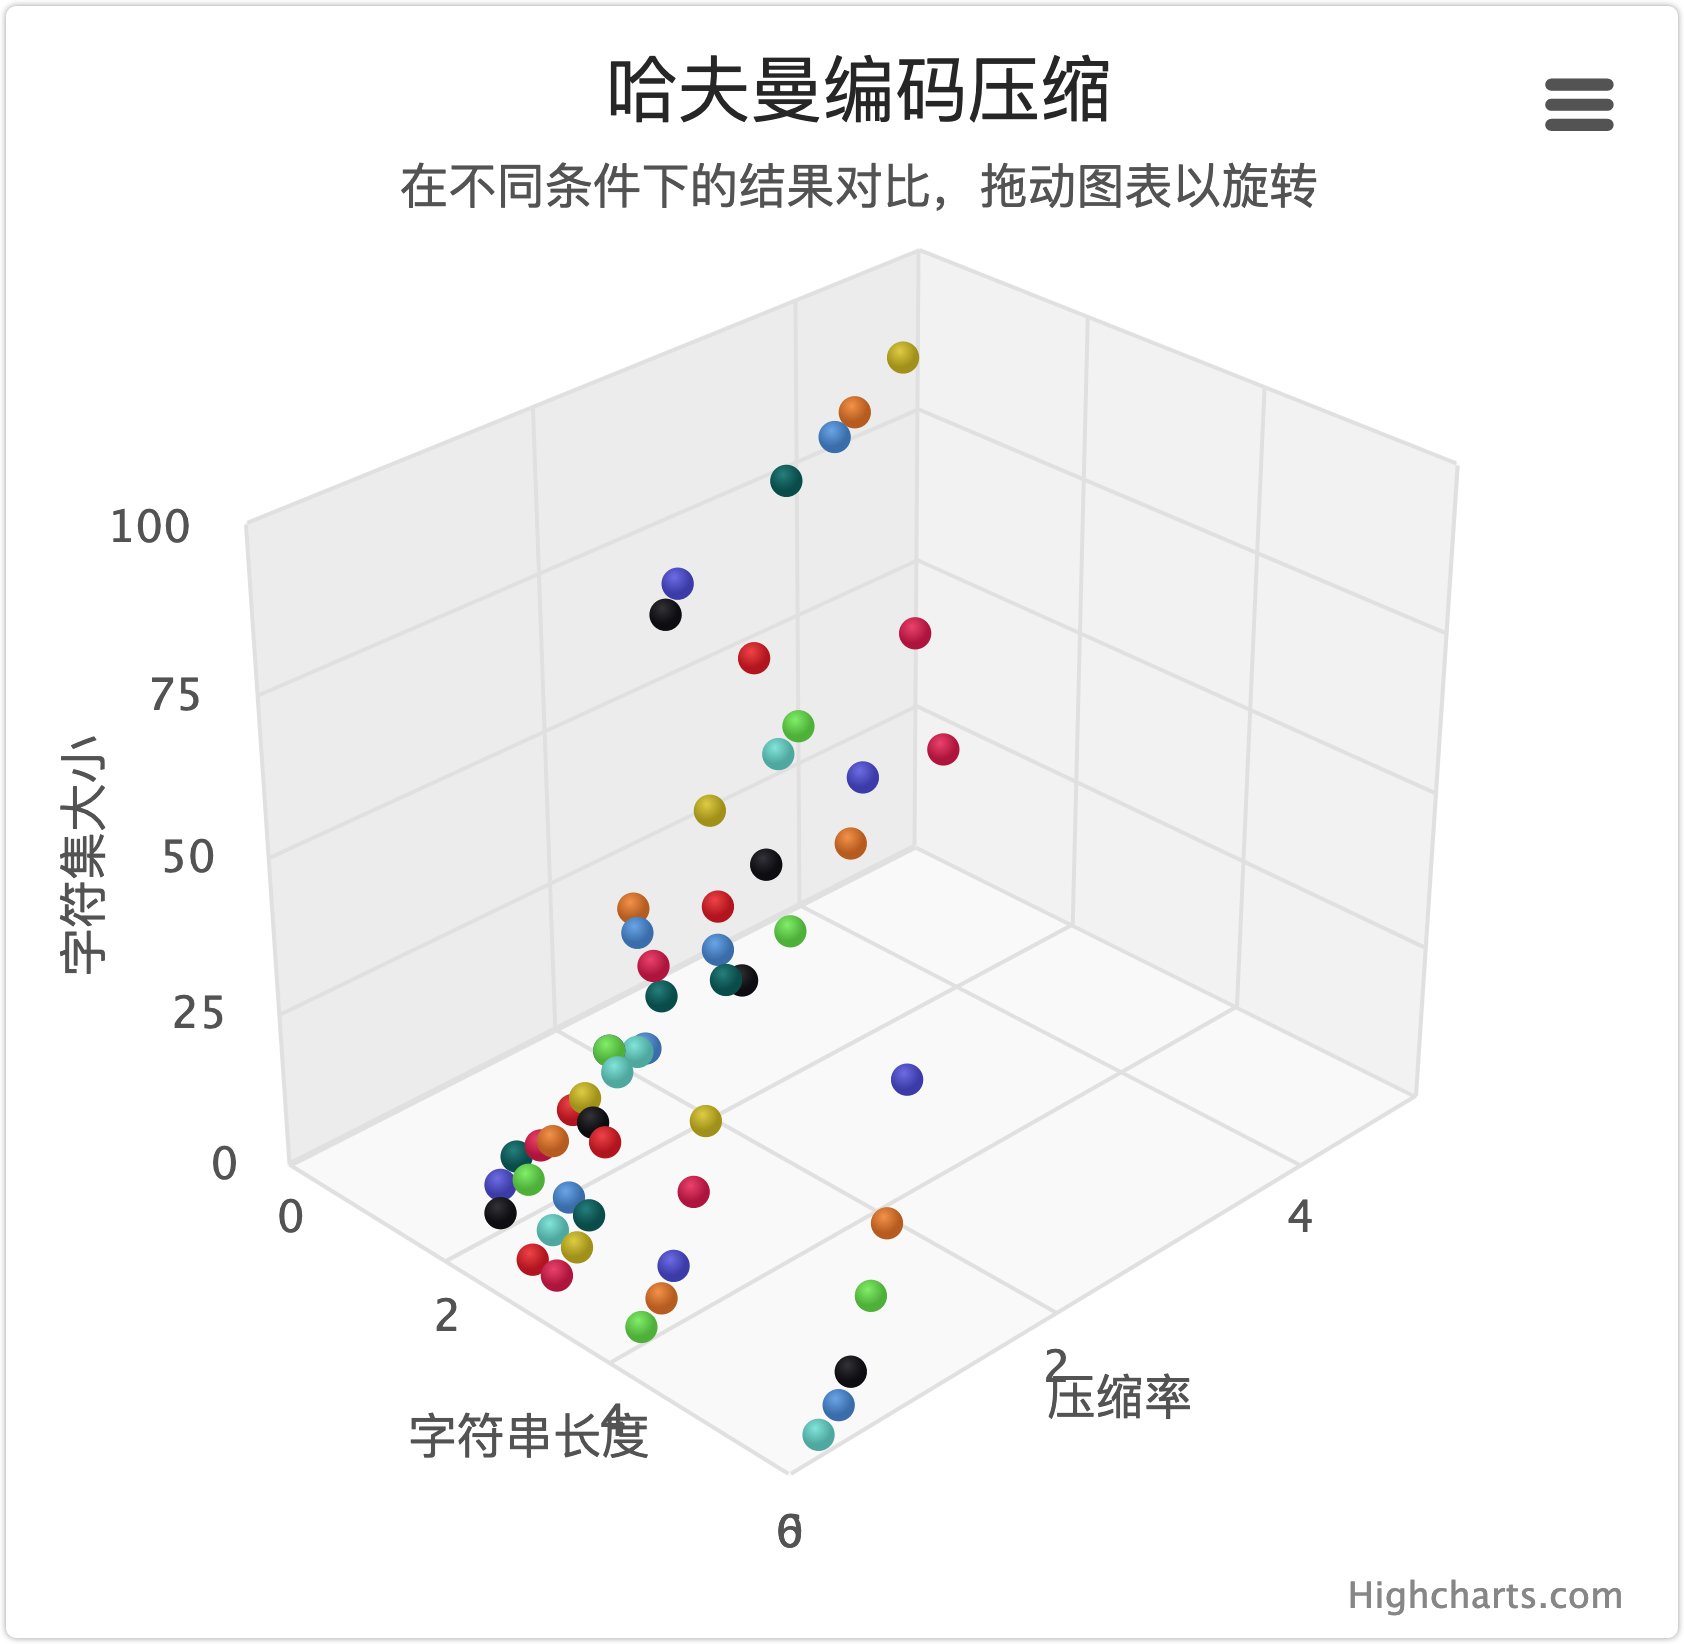
\includegraphics[width=0.9\textwidth]{./Images/pic4_2_3.png}
    
    \caption{可视化示例}
    
\end{figure}

\subsubsection{结论}

可以观察到在字符串长度较小的时候和字符集大小较大的时候压缩率有明显上升,理想情况下在字符集大小在20以内,字符串大小在100以上会有比较好的压缩效果。

\end{document}
